\documentclass[a4paper]{article}

\usepackage[english]{babel}
\usepackage[utf8]{inputenc}
\usepackage{amsmath,amssymb}
\usepackage{graphicx}
\usepackage[font={small,it}]{caption}
\usepackage[colorinlistoftodos]{todonotes}
\usepackage{hyperref}

% Använd dessa om ni vill lägga in kommentarer med \dittnamn{kommentar}
%\newcommand{\robert}[1]{\todo[color=green!40]{#1}}
%\newcommand{\yue}[1]{\todo[color=blue!40]{#1}}
%\newcommand{\martin}[1]{\todo[color=red!40]{#1}}

\oddsidemargin=0in
\evensidemargin=0in
\textwidth=6.25in
\headsep=0pt
\headheight=0pt
\topmargin=0in
\textheight=9.5in


\title{Photovoltaic effect}

% Skriv dit ditt namn.
\author{Robert Vedin \\ Yue Jiao \\ Martin Sundin}

\date{April 21, 2016}

\begin{document}
\maketitle

%\listoftodos

\section{Introduction}

The photovoltaic effect is the name of the phenomenon where a voltage appears over a p-n junction when subject to photons of sufficient energy. A p-n junction consists of a semiconductor where one part is doped with acceptor (positive) atoms and the other with donor (negative) atoms. This will cause the negatively charged electrons from the n-side to diffuse over to the p-side until the electrical potential has canceled the effect of the doping. The relation between the current $I$ and voltage $V$ is described by the {\it diode equation}. The diode equation as described in the lab paper is written as
\begin{align}\label{diode_eq}
	I(V) = I_{sat} \bigg(1 - \exp\Big(-\frac{eV}{n k_B T}\Big) \bigg)
\end{align}
where $n$ is the so called \emph{ideality factor}.

In this experiment we will studied some properties of a p-n junction solar cell. We studied the efficiency of the solar cell, the ideality factor and the limiting frequency for the current to be built in the solar cell. 

\section{Experimental procedure}

The equipment as well as the software 'Cassy lab' were set up as described in the instruction. We then proceeded to measure the current with no light-source on, at 500 points separated by 200 $\mu s$. The same procedure was repeated with the light-source placed just above the solar cell.

For the second part the software settings were set according to the instructions and the measurements were repeated, this time plotting current versus voltage as well as the power delivered by the cell.

To find out how the power delivered by the solar cell depends on the distance $d$ between the light-source and the cell, we plotted $I$ and $P$ respectively against $V$ for different values of $d$. We chose 10 equidistant values of $d$, ranging from 5 $cm$ to 50 $cm$. The acquired data were exported to Matlab in .txt format, and converted to relevant plots using the scripts that were provided next to the lab instruction. 

\section{Measurement results}

In order to derive the power dependence upon the distance from the lamp we first consider the lamp as a point which emits a power $P_0$. Some distance $r$ away from the lamp this power will be distributed over some area proportional to $r^2$ such that the intensity is $I(r) = \frac{I_0}{r^2}$ where $I_0$ is some constant. The power received by the solar cell is then obtained by multiplying the intensity with the area of the solar cell $P(r) = A \frac{I_0}{r^2} = \frac{P_0}{r^2}$, where $P_0$ is a new constant. Now since the lamp is not a point and has a non-zero radius our measured values of $d$ will not be exactly equal to $r$, rather $r = d + d_0$ such that we get $P(d) = \frac{P_0}{(d_0 + d)^2}$ where $P_0$ and $d_0$ are two fit parameters. With $P(d) = f(d)$ as described in the lab paper we get the parameter $\frac{f(d)}{f(0)}$

\begin{align}\label{eq}
	\frac{f(d)}{f(0)} = \frac{P_0}{(d_0 + d)^2} \frac{d_0^2}{P_0} = \frac{1}{(1 + \frac{d}{d_0})^2}.
\end{align}


If we consider a circuit with two components connected in series, one a voltage source with voltage $V$ \& internal resistance $R_0$ and the other a load with resistance $R$, then using Ohm's law the current through the circuit can be written as 
\begin{align}
	I = \frac{V}{R_{tot}} = \frac{V}{R_0 + R}.
\end{align}
The output power of the load we get as $I^2 R$, which if we enter $I$ as above becomes
\begin{align}
	P(R) = I^2 R = V^2 \frac{R}{(R_0 + R)^2}.
\end{align}
Finally differentiating this with respect to $R$ in order to determine the optimal load $R_{max}$
\begin{align}
	\frac{dP}{dR} = V^2 \Big ( \frac{1}{(R_0 + R_{max})^2} - \frac{2 R_{max}}{(R_0 + R_{max})^3} \Big ) = V^2 \frac{(R_0 - R_{max})}{(R_0 + R_{max})^3} = 0,
\end{align}
which is satisfied for $R_{max} = R_0$.

In order to determine the voltage $U$ at maximum power we use $U = U_0 - I R_0$ as defined on page 2 of the lab paper and write the power
\begin{align}
	P = -UI = -\frac{1}{R_0}(U_0U - U^2).
\end{align}
Differentiating this with respect to $U$ in order to maximize $P$ yields
\begin{align}
	\frac{dP}{dU} = -\frac{1}{R_0}(U_0 - 2U) = 0
\end{align}
which is satisfied for $U = \frac{1}{2}U_0$. This is not quite fulfilled in our measurements. By using Equation \ref{diode_eq} and our experimental data the relation is observed to be closer to $U \approx \frac{1}{1.33}U_0$
%\robert{Tror vi på det här?}

\begin{figure}
\centering
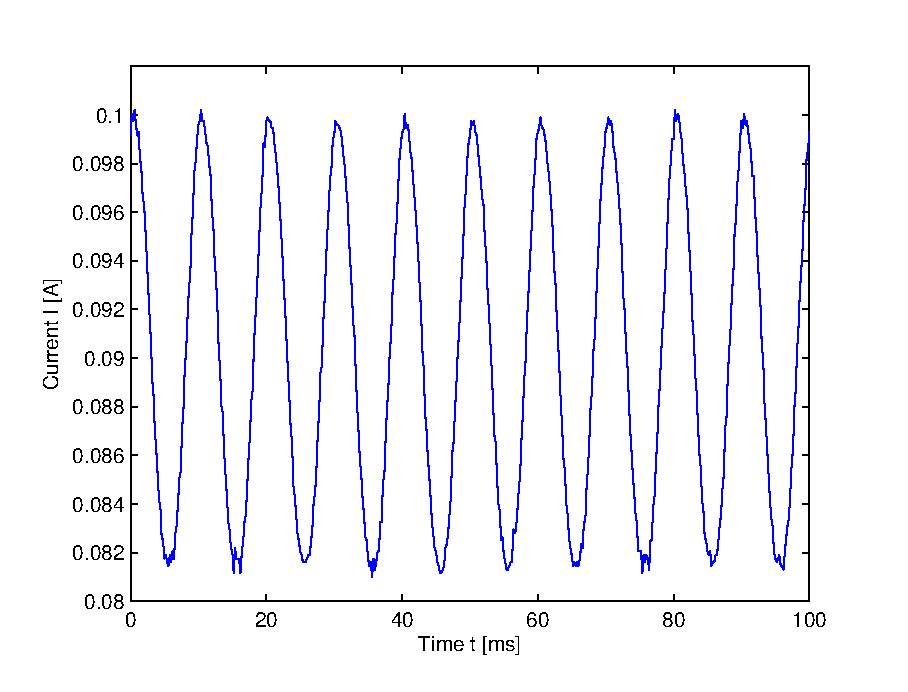
\includegraphics[scale = 0.8]{solarNoBias.eps}
\caption{\label{no_bias}This figure shows a plot of the measured current $I$ at zero-bias as a function of the time $t$. }
\end{figure}



\begin{figure}
\centering
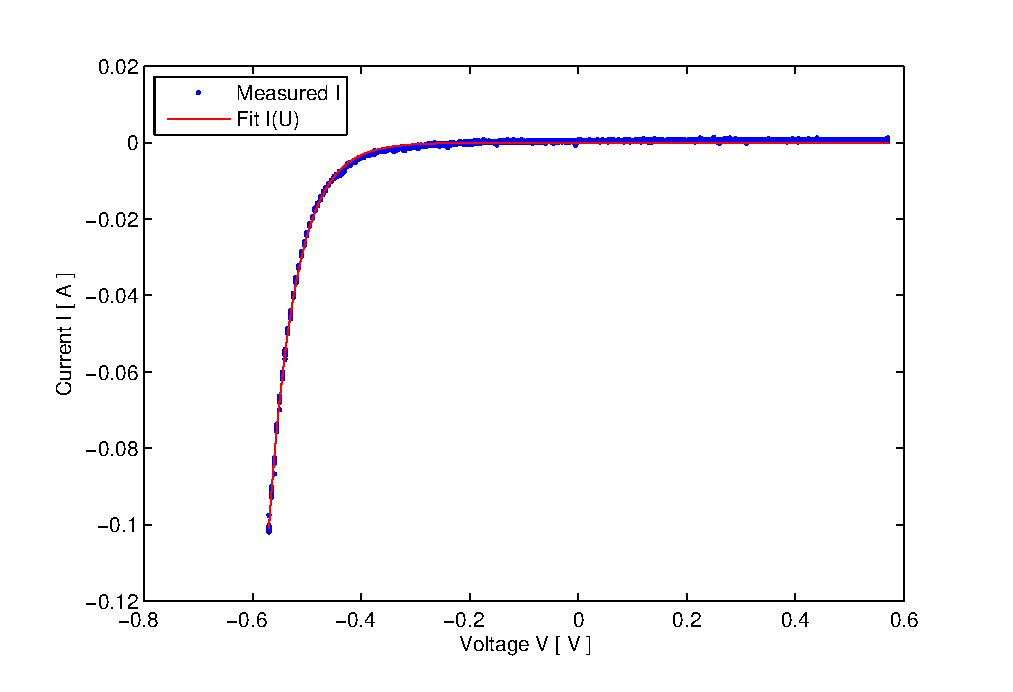
\includegraphics[scale = 0.7]{solar41.eps}
\caption{\label{solar41}This figure shows a plot of the measured current $I$ as a function of the voltage $V$ when the light-source was turned off, with the diode equation fit shown in red. }
\end{figure}


\begin{figure}[h]
\centering
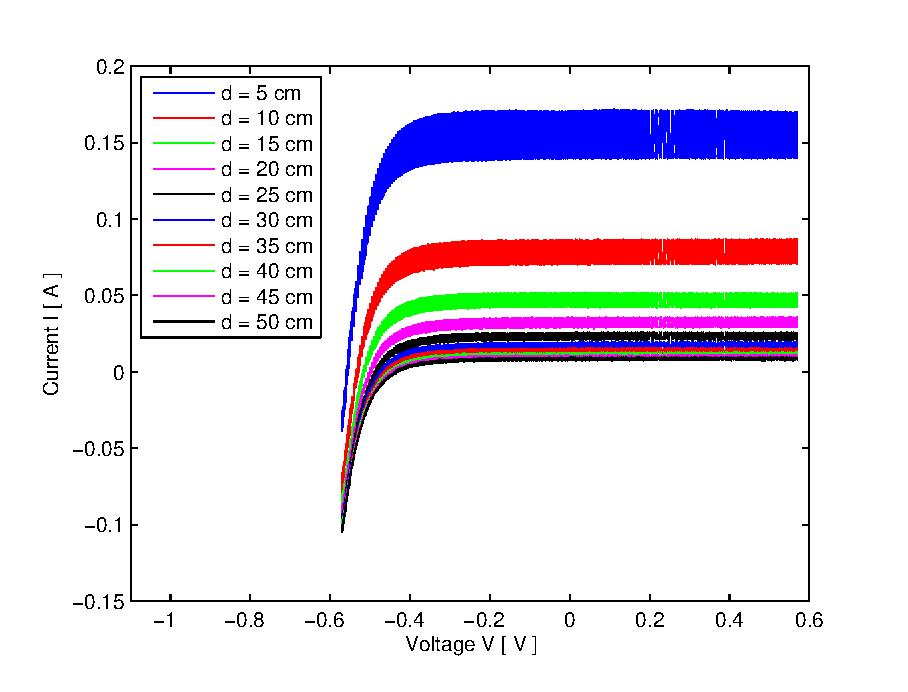
\includegraphics[scale = 0.78]{solar42IV.eps}
\caption{\label{solar42IV}This figure shows the current $I$ plotted versus the voltage $V$ for different distances $d$. Due to a lack of colors a few distances will have had to share color. Fortunately the curves are shown in the same order as indicated in the legend.}
\end{figure}


\begin{figure}[h]
\centering
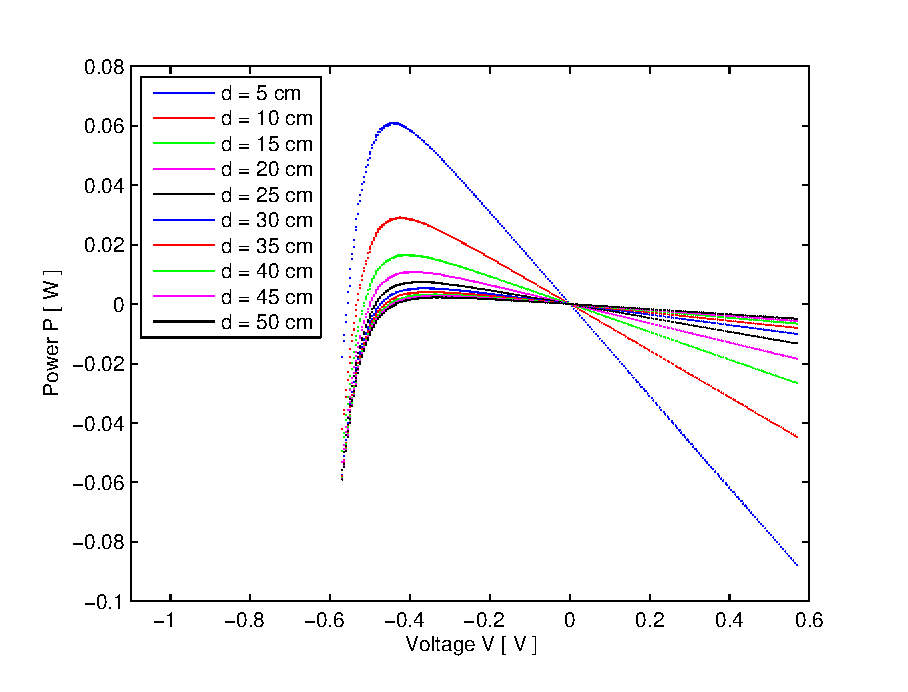
\includegraphics[scale = 0.78]{solar42PV.eps}
\caption{\label{solar42PV}This figure shows the power $P$ plotted versus the voltage $V$ for different distances $d$. Due to a lack of colors a few distances will have had to share color. Fortunately the curves are shown in the same order as indicated in the legend.}
\end{figure}


\begin{figure}[h]
\centering
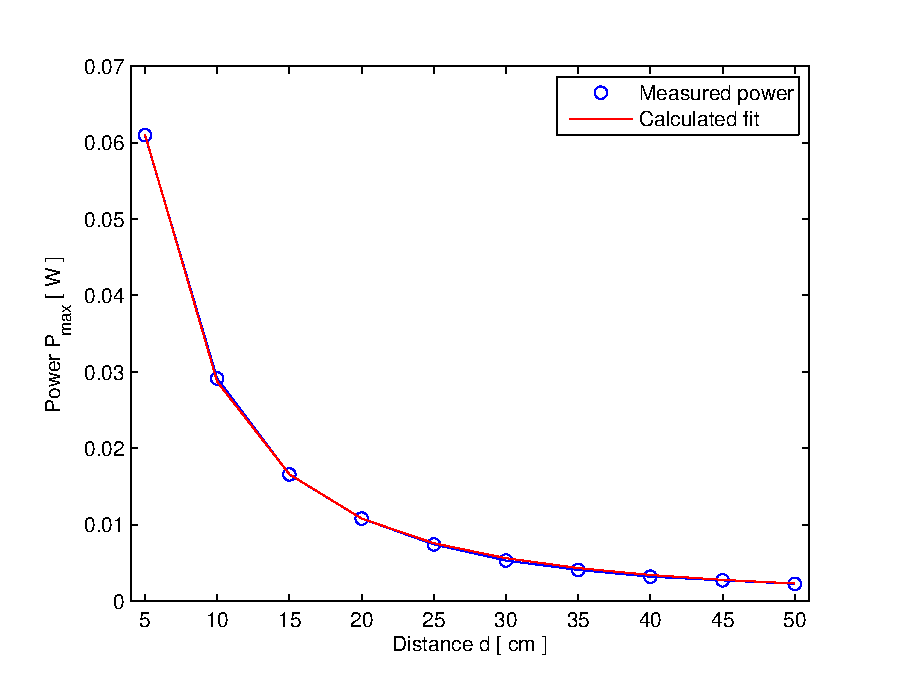
\includegraphics[scale = 0.78]{solar42Fit.eps}
\caption{\label{solar42Fit}This figure shows the maximum power $P_{max}$ plotted versus the distance $d$ and the calculated curve-fit function in shown red.}
\end{figure}


\begin{figure}[h]
\centering
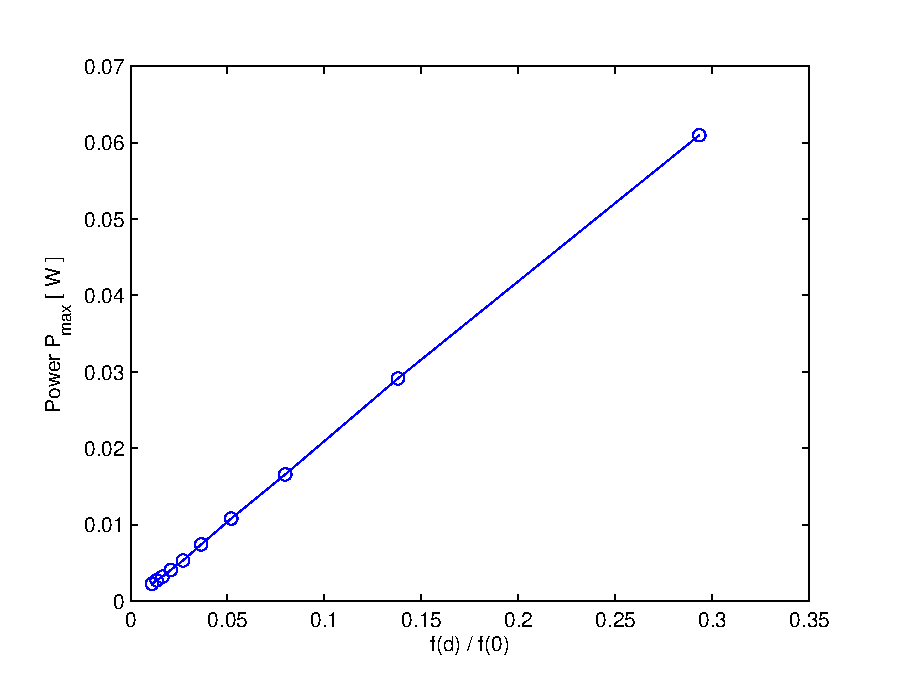
\includegraphics[scale = 0.78]{solar42Line.eps}
\caption{\label{solar42Line}This figure shows the maximum power $P_{max}$ plotted versus the parameter $f(d) / f(0)$.}
\end{figure}

\clearpage

\section{Discussion}


The lamp used in this experiment was an incandescent bulb which emits a fairly wide span of frequencies. Because of the band-gap the photovoltaic cell will be transparent to light whose frequency is too low. The limiting frequency is obtained by equating the photon energy $h f$ to the band-gap energy $E_g$ of the material. The photovoltaic cell used in this exercise was a silicon thin film, which according to a table on page 190 (Kittel, 8th edition) has a band-gap energy $E_g = 1.11 \,\mathrm{[eV]}$ at room temperature. This yields a limiting frequency
\begin{align}
	f_{lim} = \frac{E_g}{h} \approx 268.2 \cdot 10^{12} \,\mathrm{[Hz]},
\end{align}
which corresponds to a limiting wavelength $\lambda_{lim} \approx 1118 \,\mathrm{[nm]}$.

%Since the lamp runs on alternating current whose frequency is $50 \,\mathrm{[Hz]}$ and the radiated power is proportional to the current squared the power delivered to the photovoltaic cell should have a frequency twice as high.

The lamp runs on alternating current whose frequency is $50 \,\mathrm{[Hz]}$. However both of current's direction shall give the same radiated power since power is proportional to the current squared and the radiated power has no direction. So the energy the photovoltaic cell receives is too proportional to the current squared. Since the waveform of the alternating current is a sine wave so its square shall has a frequency twice as high which is exactly $100 \,\mathrm{[Hz]}$

A plot of the current at zero-bias can be seen in figure \ref{no_bias}, it appears to be a sinusoidal function of time with an estimated frequency $f \approx 100.2 \,\mathrm{[Hz]}$. The frequency was estimated by calculating the mean value $\Delta t_{mean}$ of the time-spacing between each pair of consecutive peaks. An estimation of $f$ is then obtained as $f \approx \frac{1}{\Delta t_{mean}}$.

The $IV$ characteristics of the photovoltaic cell in the case of no illumination can be seen in figure \ref{solar41}, and it appears to be a good fit to the Diode equation as described in equation \ref{diode_eq}. Using the provided MATLAB script we calculated a value for the fit-parameter $\frac{n k_B T}{e} \approx 0.0496$, and using an estimated value for the temperature $T \approx 300 \,\mathrm{[K]}$ we calculated an approximate value for the ideality factor $n \approx 1.917$.

A plot of the maximum power as a function of the distance can be seen in figure \ref{solar42Fit} and the fit appears to be fair. Figure \ref{solar42Line} shows the maximum power plotted versus the parameter $\frac{f(d)}{f(0)}$ and the plot again appears to be a good fit to the expected line.

% Behöver eventuellt inte vara med.
Using the MATLAB function fminseach we obtained an estimated value for the fit-parameter $d_0 \approx 5.91 \,\mathrm{[cm]}$ which is a reasonable value for the radius of a light bulb.



\section{Conclusions}

Using the curve showing the theoretical maximum efficiency as provided in the lab paper we estimate that the maximum occurs for $x_g = \frac{E_g}{k_B T} \approx 2.2$, yielding an optimal band-gap energy $E_g \approx 2.2 k_B T$. For a solar cell the temperature of interest is the temperature of the sun. This temperature we found on \href{https://www.wolframalpha.com/input/?i=temperature+of+the+sun}{WolframAlpha} to be $T \approx 5780$ [K]. With this the optimal band-gap energy becomes 
\begin{align}
	E_g \approx 2.2 \cdot 1.38 \cdot 10^{-23} \cdot 5780 \,\mathrm{[J]} \approx 1.10 \,\mathrm{[eV]},
\end{align}
looking again to the table on page 190 of Kittel (8th edition) this appears to  be a good match for the band-gap energy of the silicon crystal.

To estimate the efficiency of the solar cell used in the lab we start by estimating that the power output of the light-bulb $P_b \approx 50$ [W]. The intensity at some distance $d$ is then determined in the same way as was used to derive equation \ref{eq} such that
\begin{align}
	I(d) = \frac{P_b}{A_s(d)}.
\end{align}
Where the area $A_s(d) = 2 \pi (d_0 + d)^2$ is the area of a half-sphere of radius $d_0 + d$. The solar cell has some area $A_c$ and we obtain the power delivered to the solar cell as
\begin{align}\label{p_in}
	P_{in}(d) = \frac{A_c}{A_s(d)}P_b.
\end{align}
We did not measure the area of the solar cell and so we will use the estimated value $A_c \approx 10 \, [\mathrm{cm^2}]$ and the parameter $d_0$ is the same fit-parameter as was used in equation \ref{eq}.

Using equation \ref{p_in} we calculate the efficiency $\eta(d) = \frac{P_{out}(d)}{P_{in}(d)}$ for each measured value of $d$ and then estimate the efficiency as the mean value of these. This yields $\eta_{mean} \approx 0.0865$ which unfortunately does not fit very well at all with the theoretical upper limit as provided in the lab paper. 


\end{document}


